\chapter{THE MODULARIZED OFDM STACK}
\label{chap:ofdm-stack}

%%%%%%%%%%%%%%%%%%%%%%%%%%%%%%%%%%%%%%%%%%%%%%%%%%%%%%%%%%%%%%%%%%%%%%%%%%%%%%%

\section{The goal}

Ideally, we wish to achieve a level of abstraction over the physical layer that
allows us to operate at the level of bit-streams. We would like to transmit the
bits with almost no knowledge of the underlying layer and mechanism. Suppose
bits were stored as arrays of \lstinline!char! elements, we would like to
transmit them with a single function call:

\begin{lstlisting}
	char *bits;
	// ... fill in the array
	transmit(bits);
\end{lstlisting}

Underlying this, there needs to be configurability. That is, if desired, we
should be able to break the abstraction and set options on the transmitter and
receiver. One way of doing this might be through a configuration file. But this
would mean that we cannot change parameters dynamically. So the underlying
framework should allow us to access internals in the code, if desired:

\begin{lstlisting}
	double gain = get_transmit_gain();
	if(gain != 25) {        // Change gain to 25.
		set_transmit_gain(25);
	}
\end{lstlisting}

In order to achieve this, we need to have a well-abstracted and modularized
code base. The data should be disconnected from the code to the maximum extent
possible. Different components of the code should be loosely coupled, that is,
there should be minimal interdependence between different modules, and they
should be maximally self-contained.

While, at present, the OFDM stack does not meet this ideal, one may at least
say that it has plotted itself a course and is well on its way.

%%%%%%%%%%%%%%%%%%%%%%%%%%%%%%%%%%%%%%%%%%%%%%%%%%%%%%%%%%%%%%%%%%%%%%%%%%%%%%%

\section{The modules}

The program has been functionally broken up into modules, as shown in
figure~\ref{fig:modules}.

\begin{figure}[h]
	\centering
	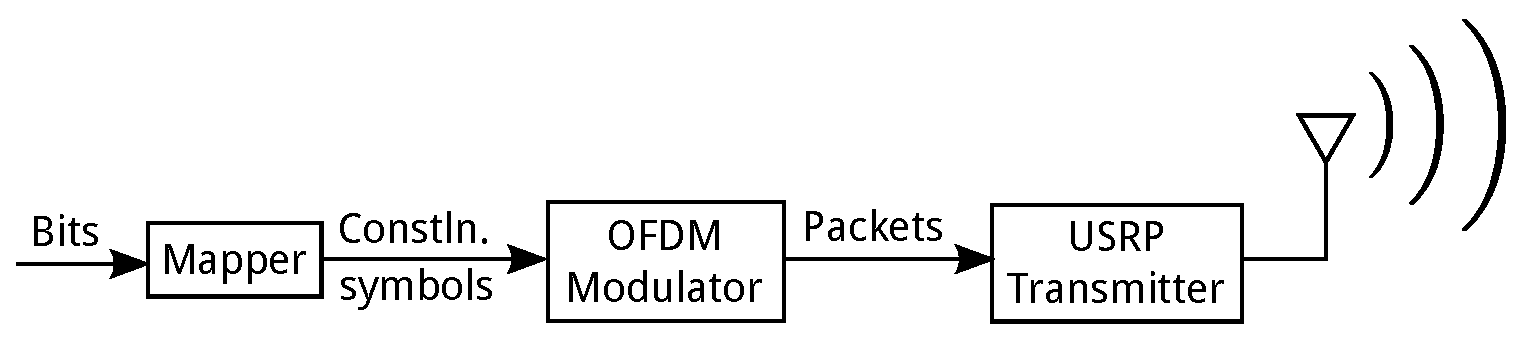
\includegraphics[width=0.8\textwidth]{transmitter-modules}
	\includegraphics[width=0.8\textwidth]{receiver-modules}
	\caption{Modules present in the OFDM stack}
	\label{fig:modules}
\end{figure}

A more detailed description of each of these modules follows.

\subsection{The mapper}

The mapper converts a sequence of bits into one of complex symbols. The reason
this has been kept outside of the OFDM framework is that different applications
have different requirements on the kinds of complex symbols generated.

Mapping may be performed on a coded bit stream, in which case it may be
sufficient to use a standard constellation to perform mapping. But in the
implementation of DPC, for example, we pre-subtract the expected interference
from another user. As a result, we do not transmit any fixed constellation
points. Any point in the available complex plane may be transmitted as a
symbol.

It is therefore best to allow for different kinds of mappers. In the interest
of keeping the OFDM framework loosely coupled with the mapping framework, the
two have been made into separate modules. The default mapper can now be
`unplugged' and a new, custom-defined mapper can be `plugged in' to the code.

\subsection{The OFDM Modulator}
\label{subsec:ofdm-modulator}

The OFDM Modulator converts a sequence of complex symbols into a sequence of
packets. Several configuration details come into play here, such as the number
of symbols that go into each frame, details of the preamble used in the frame,
etc.

In order to maintain a list of these values that can be used by the various
functions that fall under the ambit of the OFDM Modulator, the modulator has
been made into a class. The data members of the class allow for encapsulation
and abstraction, so that the settings are exposed for change only if desired.

A set of default parameters are automatically loaded when the object is
instantiated. Following this, settings can be changed by setting them manually
if desired. This can be done directly by assignment, since all data members are
public. After this, the object has to be initialized using the
\lstinline!initialize()! member function. This allocates memory and creates
\lstinline!fftw_plan!s. In a multi-threaded environment, this operation is not
thread-safe, and therefore must be completed before thread-creation.

In the transmit loop, the \lstinline!modulate()! call does the job of making
the symbols passed to it into packets. It returns a packet, which is a sequence
of time-domain complex symbols that can be transmitted using some sort of
transmitter.

\subsection{The USRP Transmitter}
\label{subsec:usrp-transmitter}

The USRP Transmitter module is an encapsulated version of the UHD API for
transmission. As described in subsection~\ref{subsec:ofdm-modulator}, some
default parameters are loaded upon instantiation, which can be changed later.
Further, the \lstinline!add_options()! member function can be used to let the
module add its own set of options to the command line, via the
\lstinline!boost! \lstinline!program_options! module. All this must be
followed up with an \lstinline!initialize()! call.

The transmitter uses the \lstinline!transmit()! function to transmit symbols.
Usually, one packet of complex symbols (as received from the OFDM Modulator) is
transmitted at a time. However, there is really no such restriction. The
transmitter can be used independently of the OFDM modulator to transmit any
sequence of complex symbols.

\subsection{The USRP Receiver}
\label{subsec:usrp-receiver}

The USRP Receiver module is similar to the USRP Transmitter in all respects.
The \lstinline!receive()! call is used to receive a desired number of complex
symbols from the USRP.

\subsection{The OFDM Demodulator}

The OFDM Demodulator is the least independent of all the modules. It is also
the heaviest in terms of computational requirement and code size. The primary
reasons for the lack of its independence are the stringent requirements of the
timing analyser, given its working mechanism. It has a specific requirement on
the buffer size. Furthermore, in order to decrease the burden on the timing
analyser, we implemented frame-discarding, as described in
subsection~\ref{subsec:frame-discard}. This resulted in the use of the
unwieldy variables \lstinline!num_left_to_search! and
\lstinline!num_to_acquire!. These variables inevitably decrease the level of
independence of this module, because they force it to become coupled with the
process of acquisition of symbols (which is really different module's work), by
definition.

This module provides the \lstinline!demodulate()! member function to detect
whether or not packets are present in the given buffer, and if they are, then
to demodulate them and return a set of received complex symbols that should
have come from transmitted constellation points.

%%%%%%%%%%%%%%%%%%%%%%%%%%%%%%%%%%%%%%%%%%%%%%%%%%%%%%%%%%%%%%%%%%%%%%%%%%%%%%%

\section{Limitations}

While the modularized implementation has enabled plugging and unplugging of
various modules, there are still many things that this framework cannot do.

\subsection{Using two different kinds of frames}

It may sometimes be desirable to use two different kinds of frames, for eg.\ a
long data frame for transmitting information, and a short acknowledgement
frame, to tell the other side that a packet has been received. While the basic
structure is present for making use of two different kinds of frames, possibly
with different preambles or data masks, the implementation of the same is not
easy and requires some work on the part of the developer.

Currently, it is possible to create two or more different OfdmModulator and
OfdmDemodulator object pairs, and then manually specifying a different preamble
or data mask for each pair. Since all data members are public, they can be
directly changed after instantiation. An \lstinline!initialize()! call will
then allocate requisite memory, create \lstinline!fftw_plan!s and so on.

Modulation too, should not be a hassle. However, when calling the demodulate
function, there is some amount of coupling between the calling program and the
demodulator in the form of \lstinline!num_left_to_search! and
\lstinline!num_to_acquire!. If the \lstinline!frame_size!s of the two types
of frames are different, then during packet detection, we may get different
values of \lstinline!num_left_to_search! and \lstinline!num_to_acquire!
from each demodulator object. We would then have to create a temporary buffer
to manage the different requirements of \lstinline!num_left_to_search! and
\lstinline!num_to_acquire! for the two demodulators.

\subsection{Using single precision}

It is currently not possible to use single precision instead of double
precision, because the FFTW module in its present configuration uses only
double precision. While this by itself would not prevent us from using single
precision elsewhere, issues arise because at present, there are
\lstinline!reinterpret_cast!s between our flexible \lstinline!Complex! and
FFTW's less flexible \lstinline!fftw_complex! data types.

In order to use single precision everywhere, there is a need to refactor the
usage of FFTW, using preprocessor tricks to switch between
\lstinline!fftw_complex!, the double precision implementation and
\lstinline!fftwf_complex!, the single precision implementation, depending on
the value of a preprocessor variable.

\subsection{Dynamically changing parameters}

At present, changing parameters, such as the USRP transmit gain, dynamically
during runtime is not easy. This is because the USRP parameter-setting
functions are currently coupled with the \lstinline!initialize()! call.
A re-initialization would cause several variables to get \lstinline!malloc!ed
again, with unknown side-effects, and is not viable at this time.

There is a need to decouple the initialization of the USRP from the process of
extracting parameters from \lstinline!program_options! and from the process of
setting parameters on the USRP.
